\section{Anhang: Screenshots der fertigen App}

Hier werden Screenshots der finalen Anwendung mit kurzen Bildunterschriften eingebunden.

\begin{figure}[H]
  \centering
  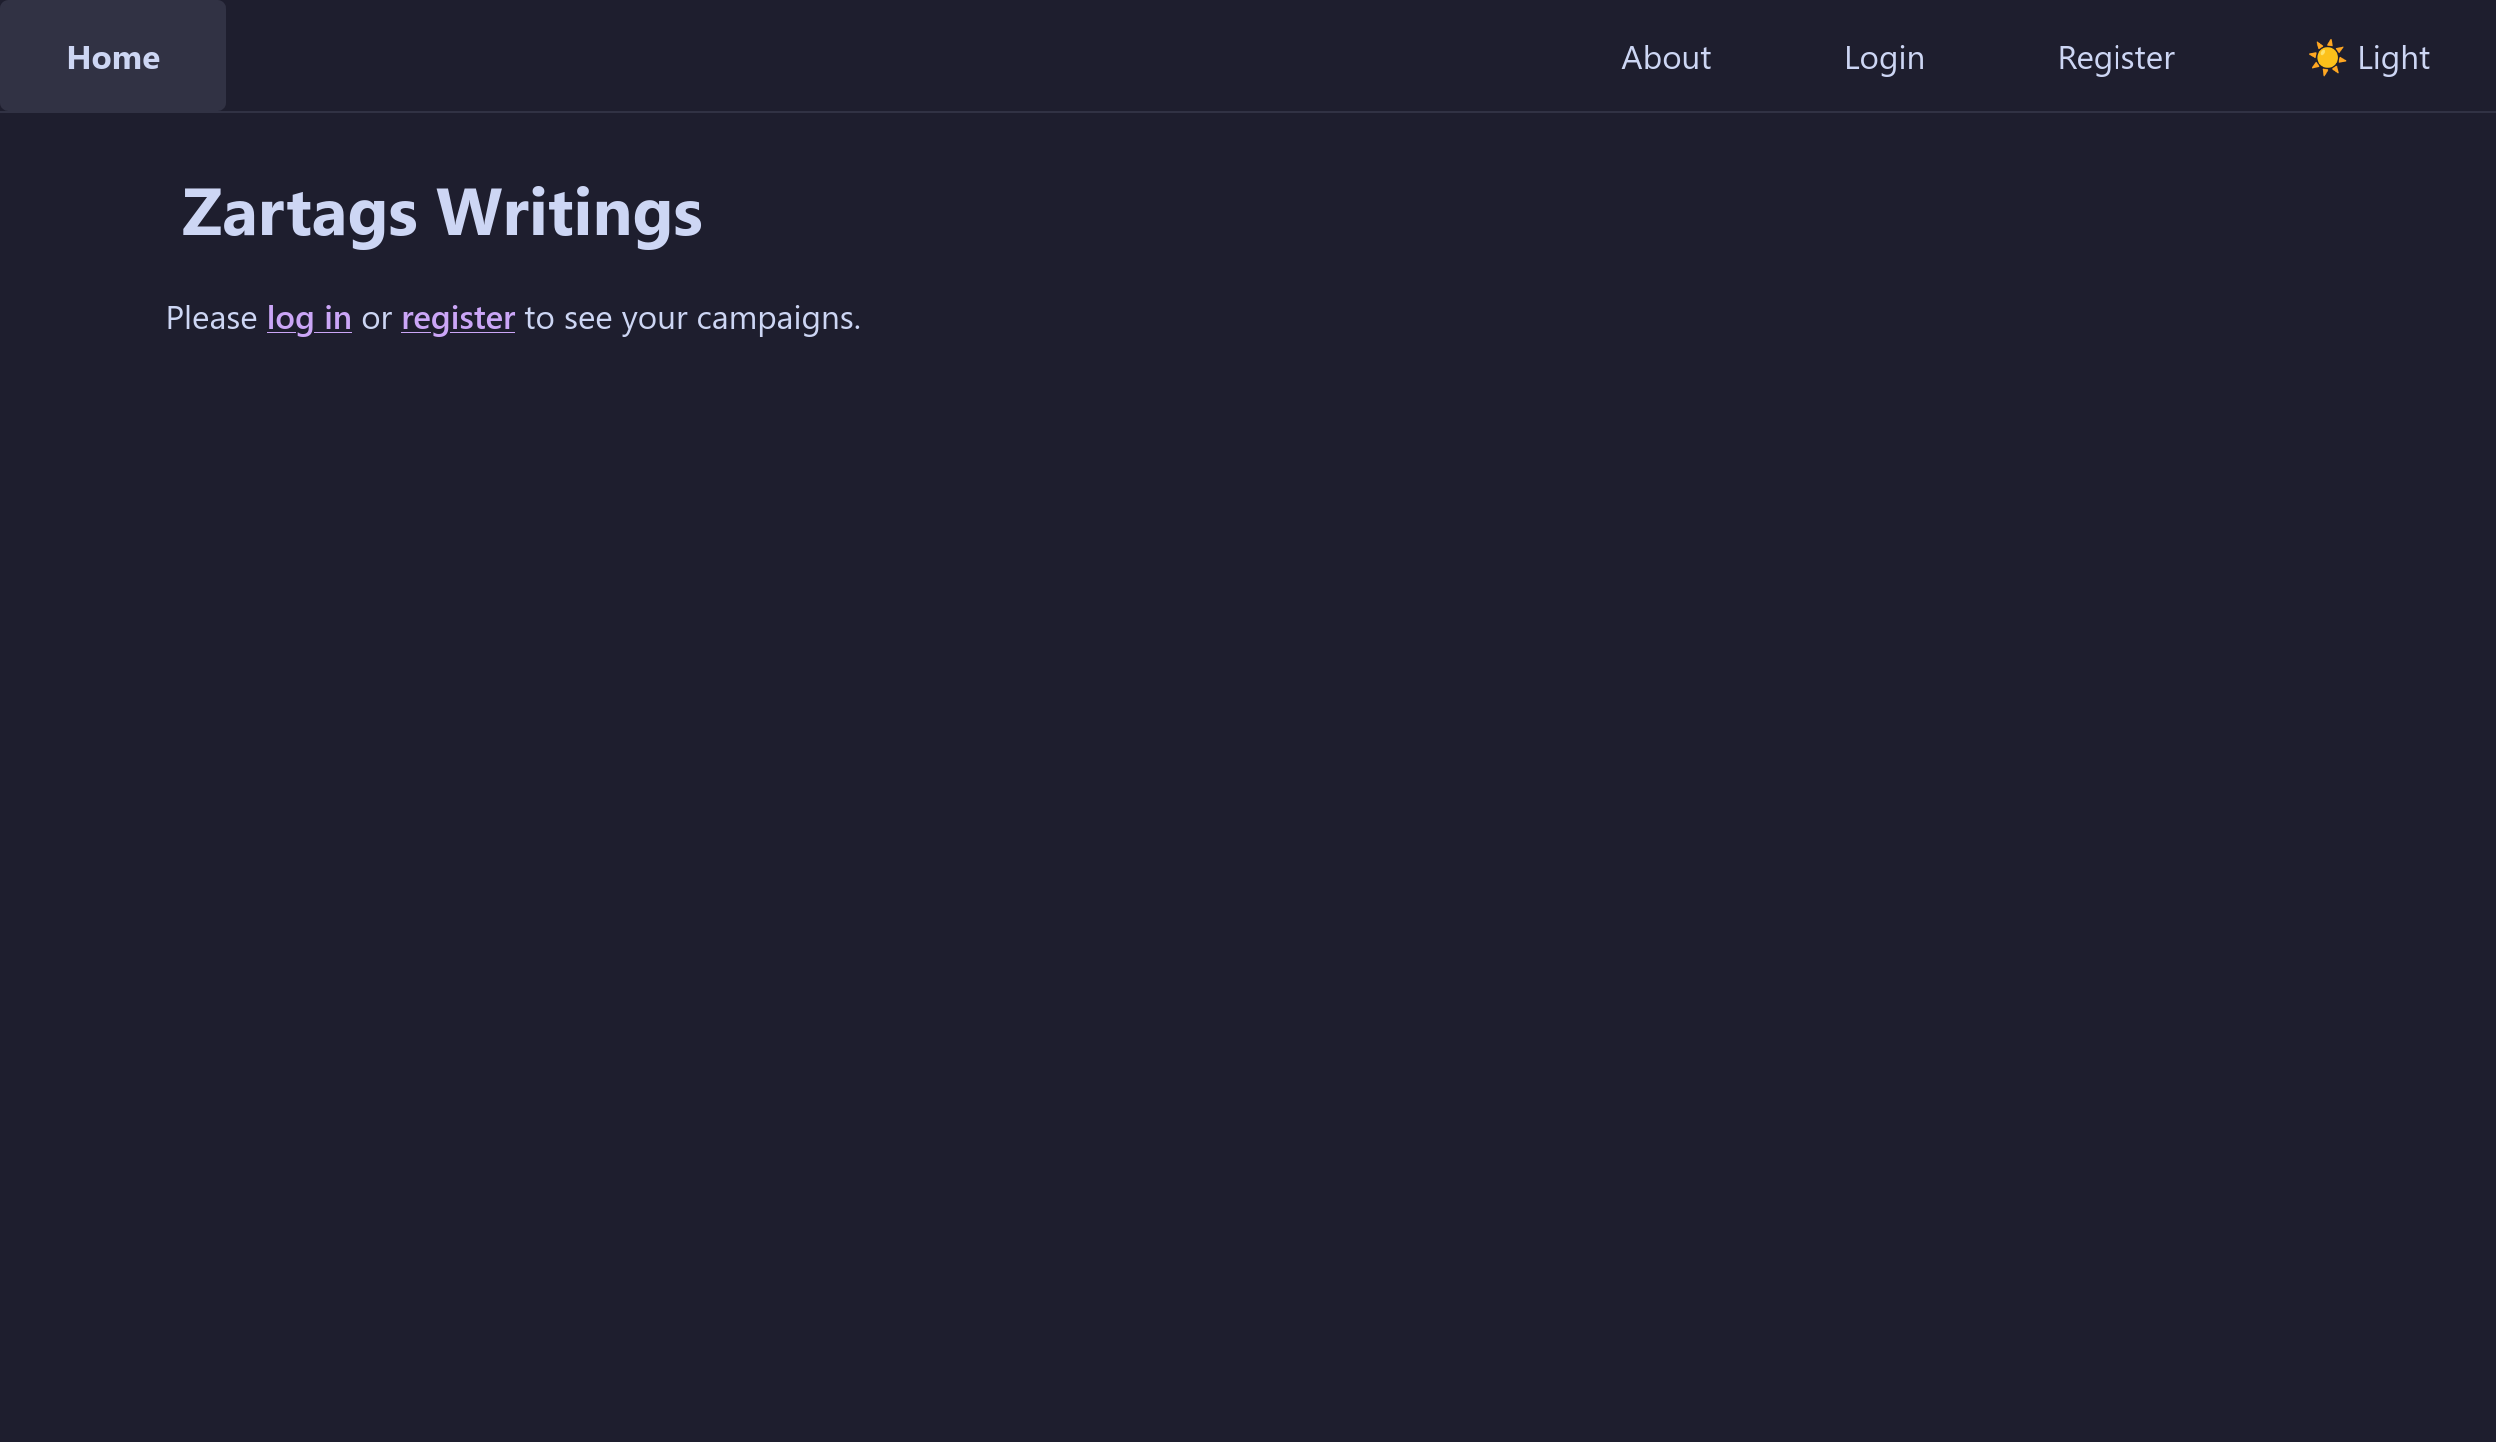
\includegraphics[width=0.92\textwidth]{media/Home_Default.png}
  \caption{Startseite ohne Login (Home Default)}
\end{figure}

\begin{figure}[H]
  \centering
  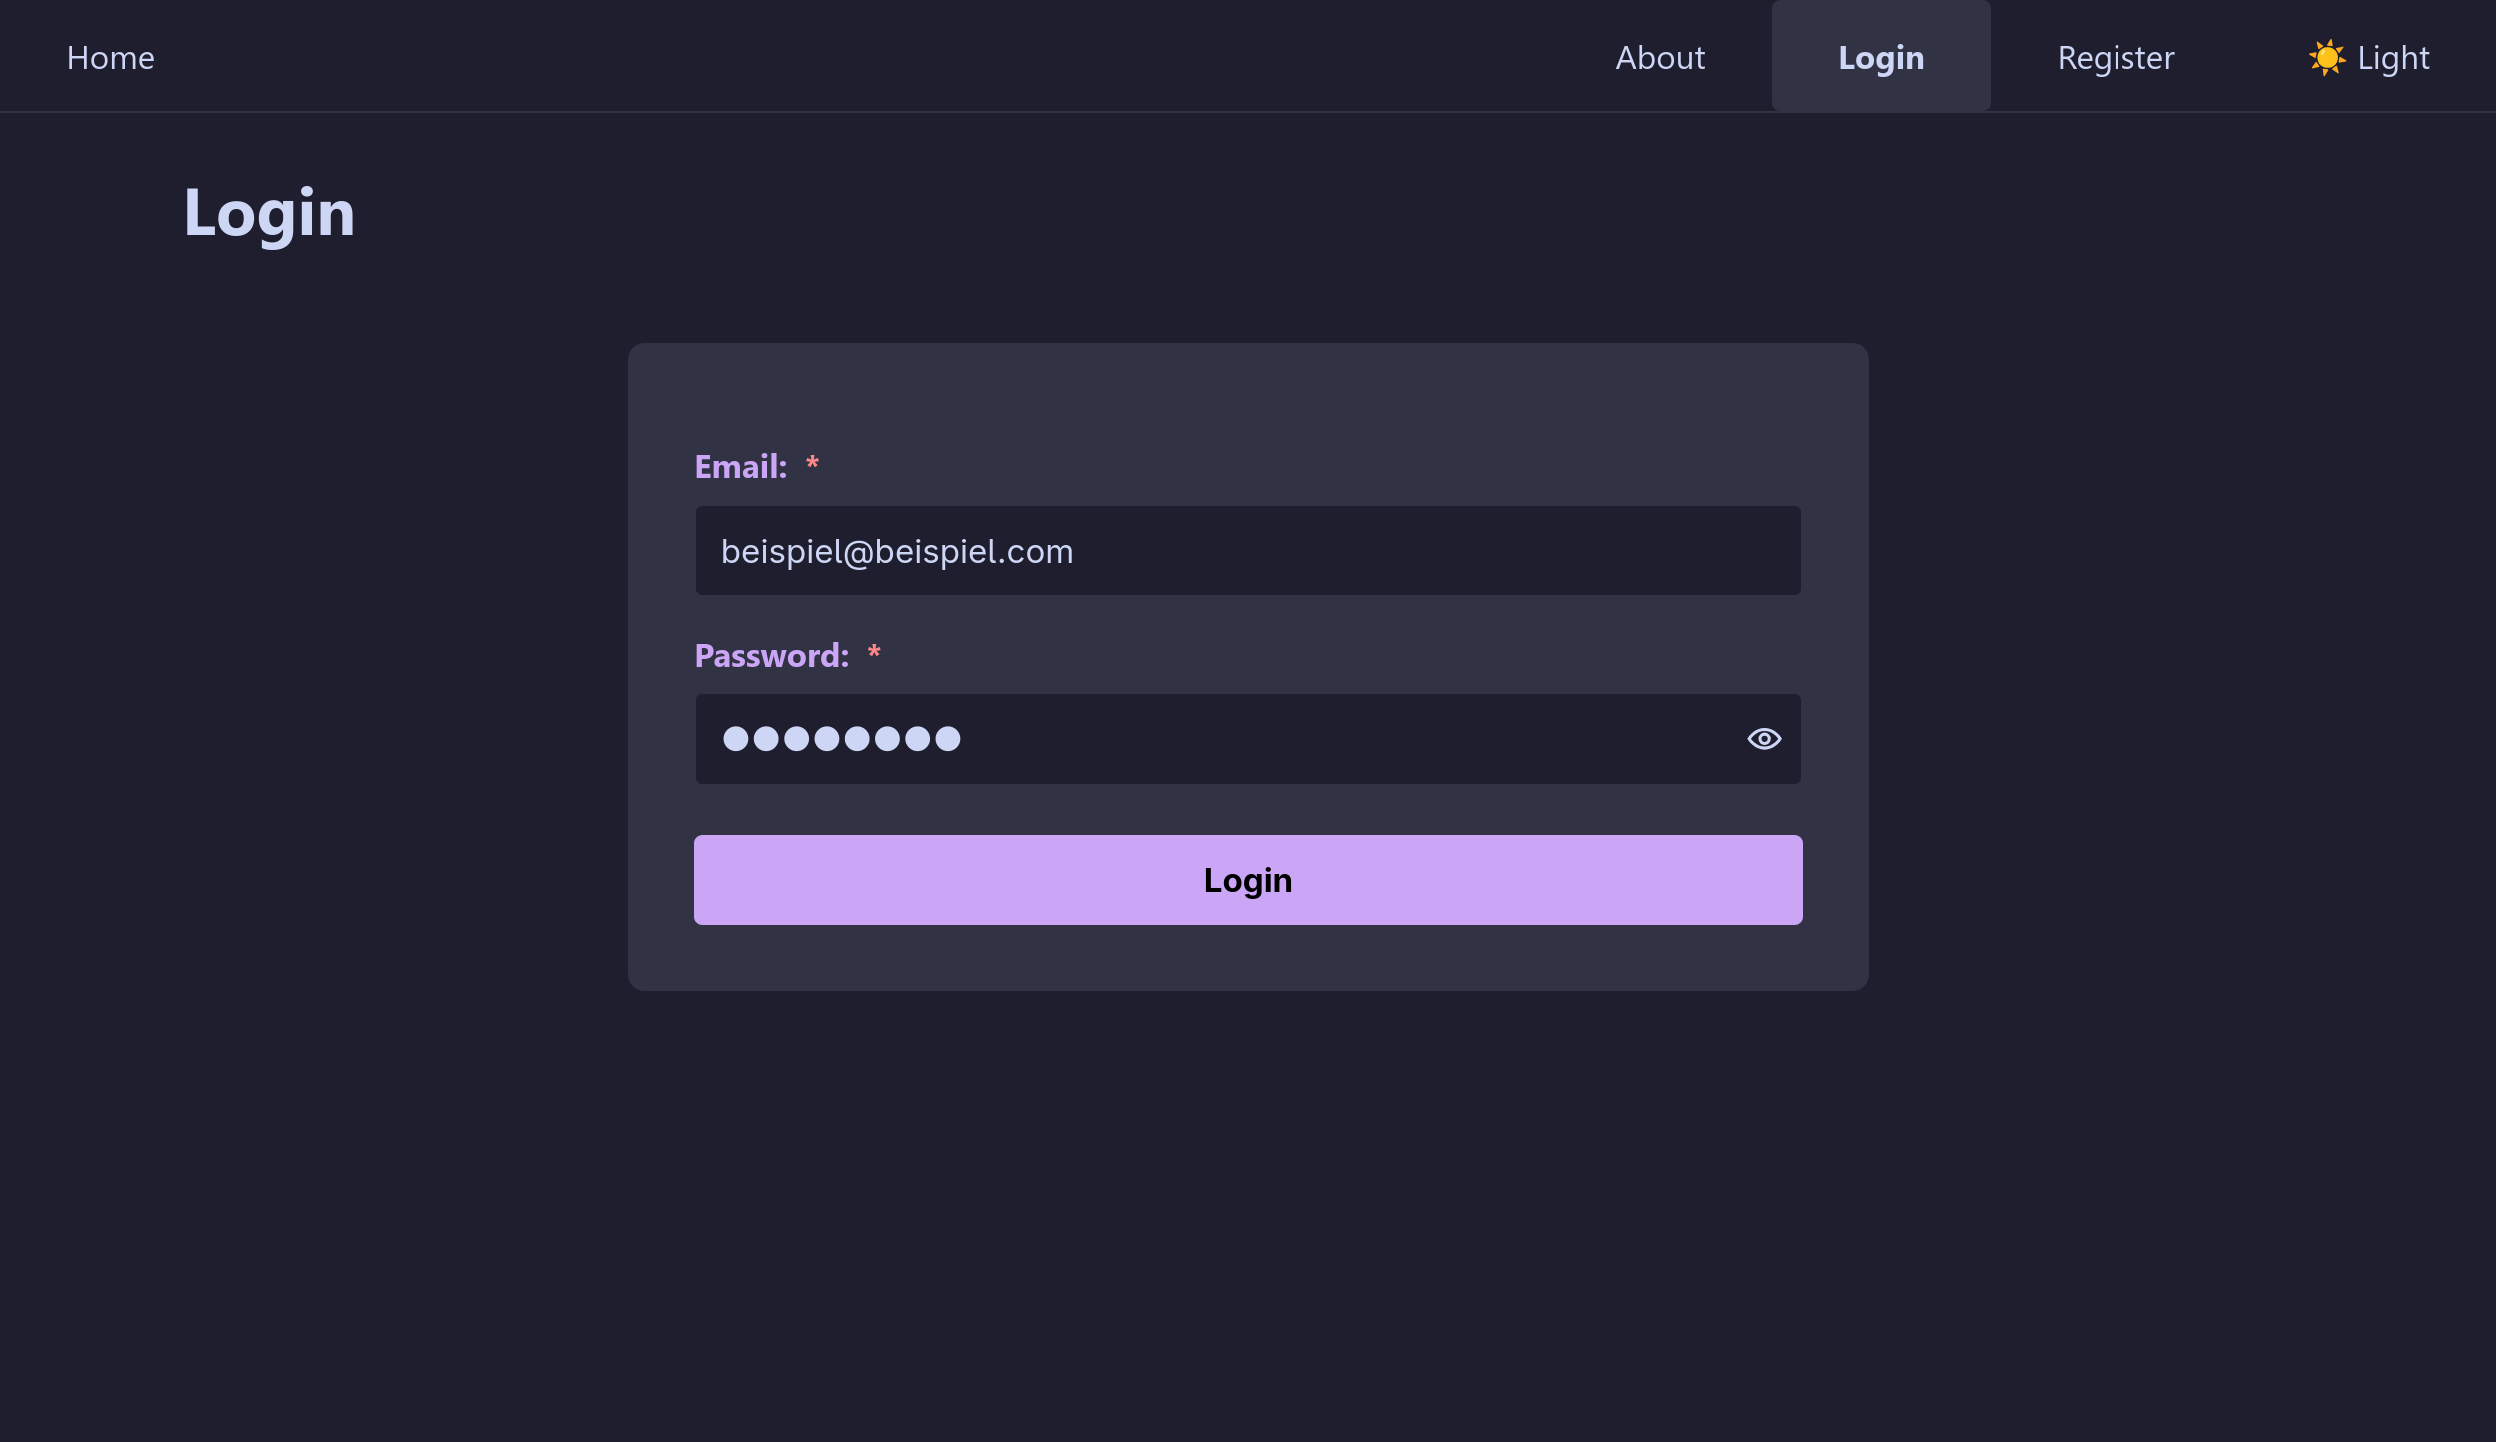
\includegraphics[width=0.92\textwidth]{media/Login_Page.png}
  \caption{Login-Seite}
\end{figure}

\begin{figure}[H]
  \centering
  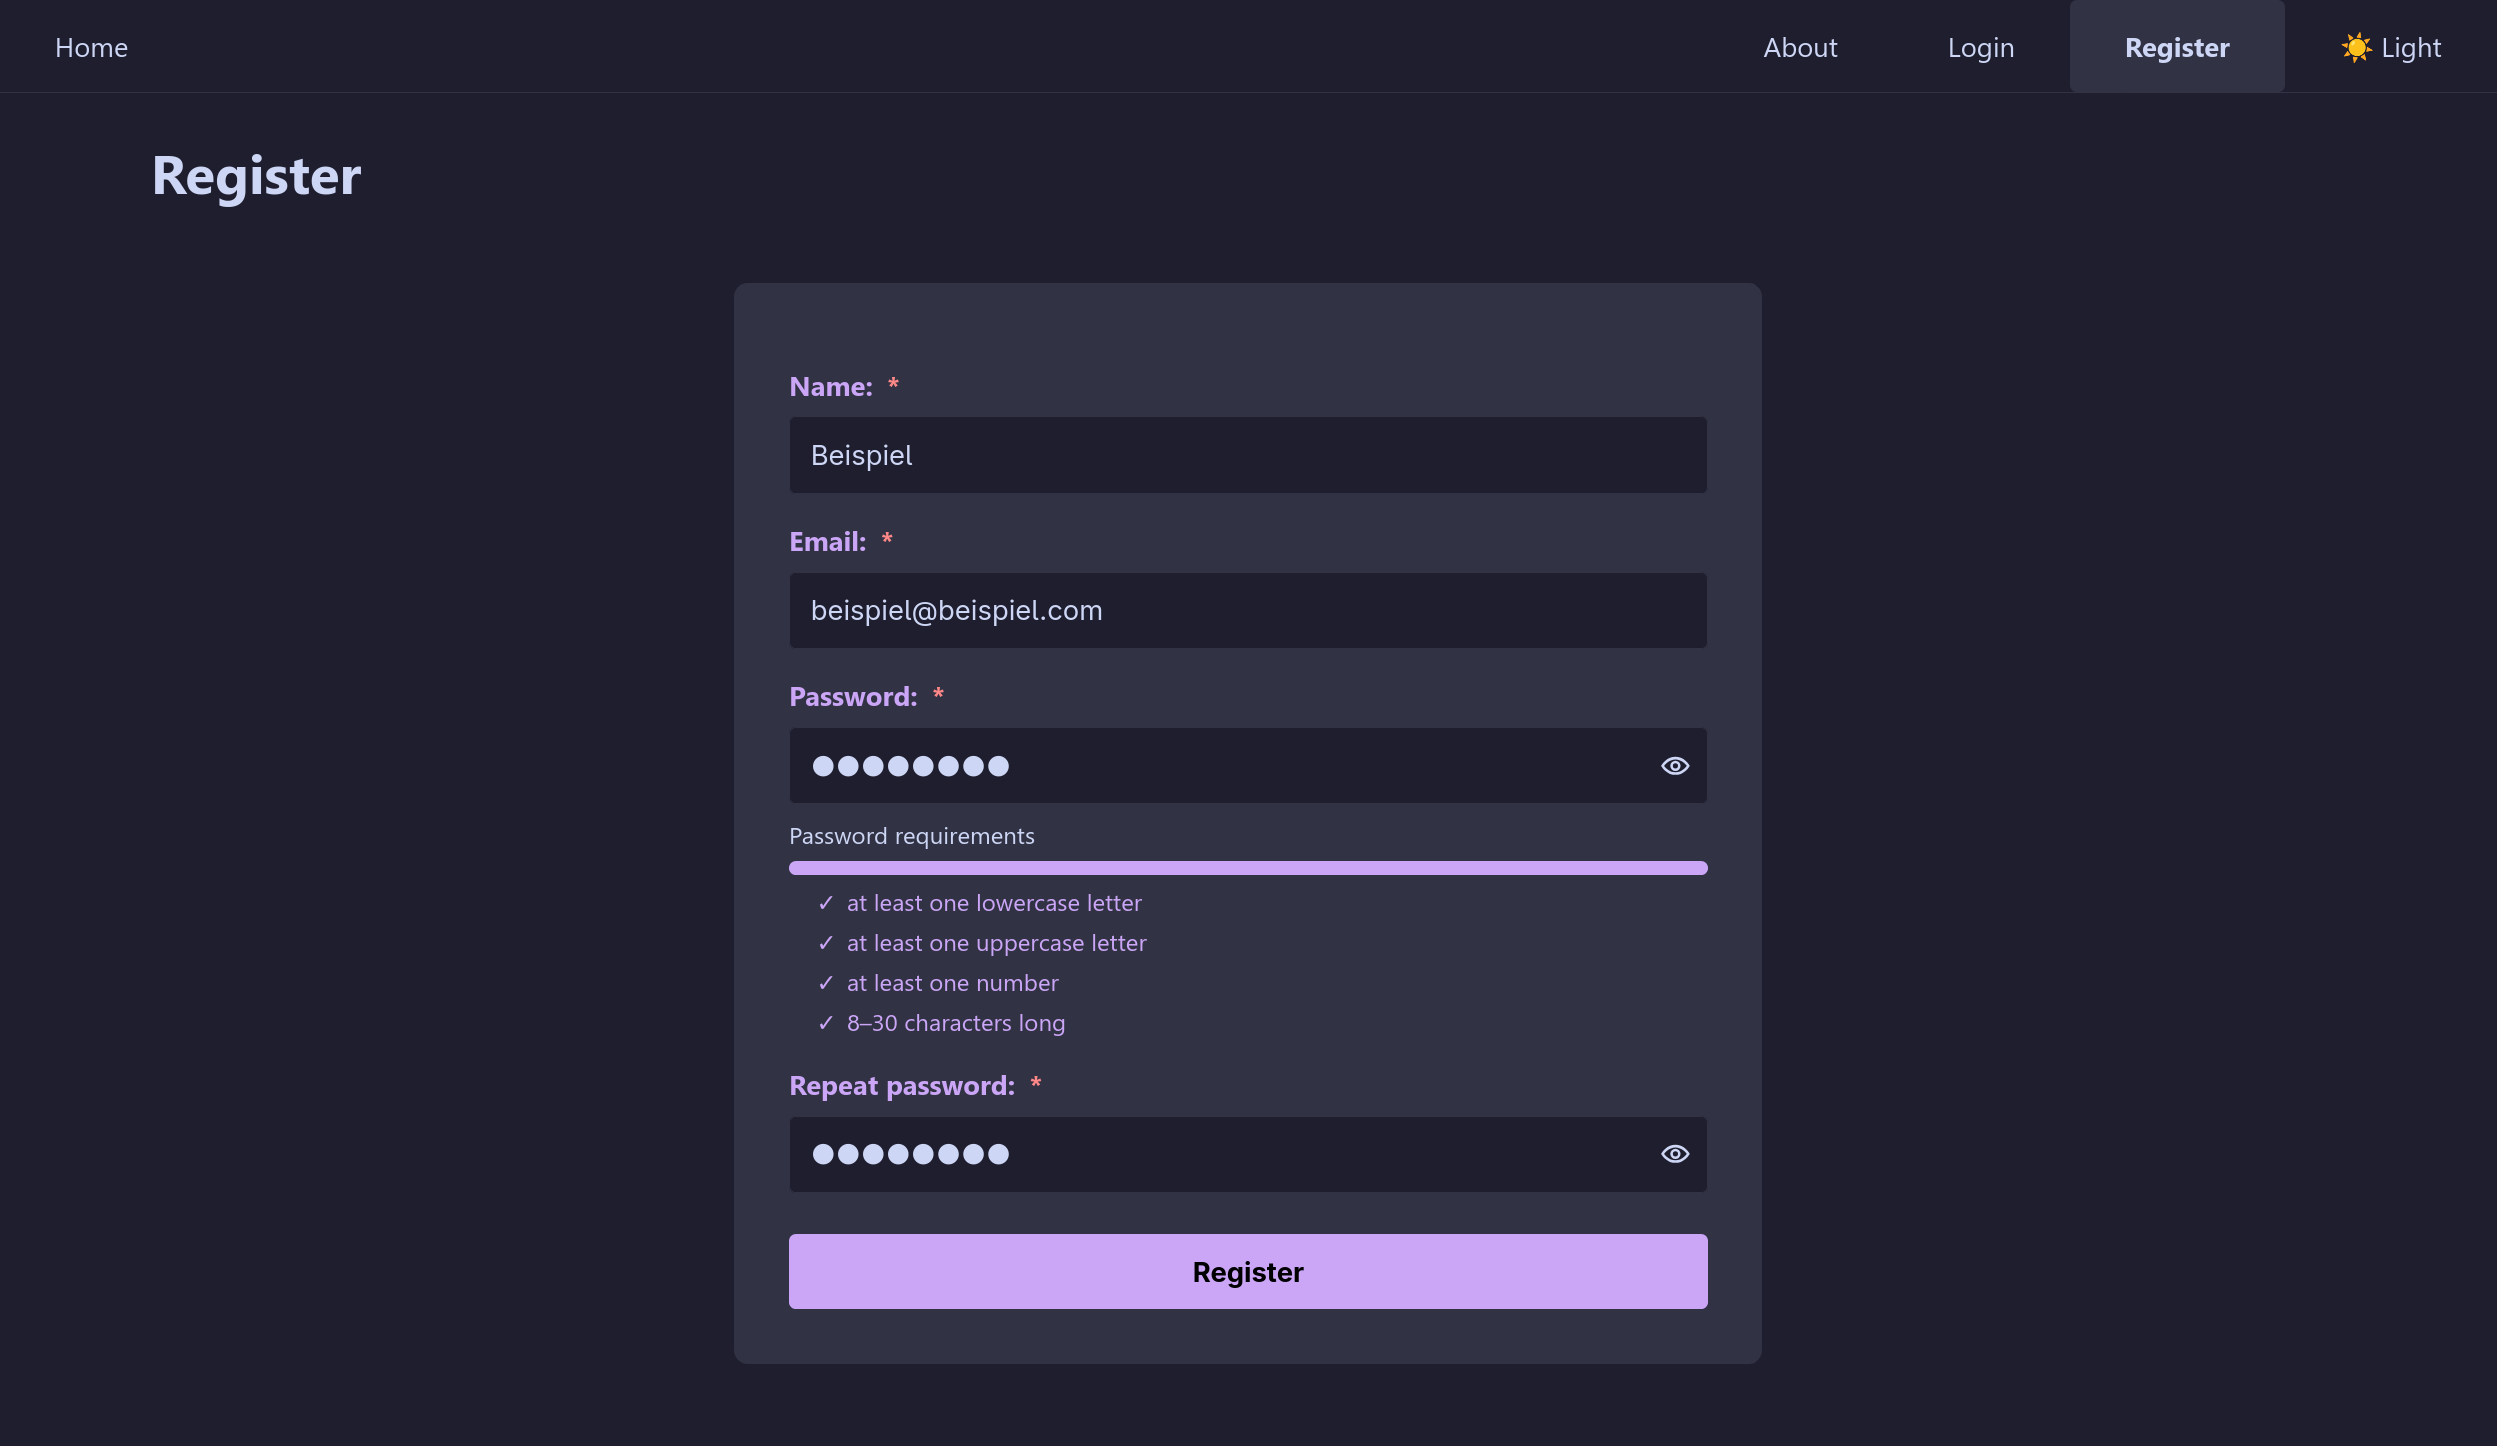
\includegraphics[width=0.92\textwidth]{media/Register_Page.png}
  \caption{Registrierungsseite}
\end{figure}

\begin{figure}[H]
  \centering
  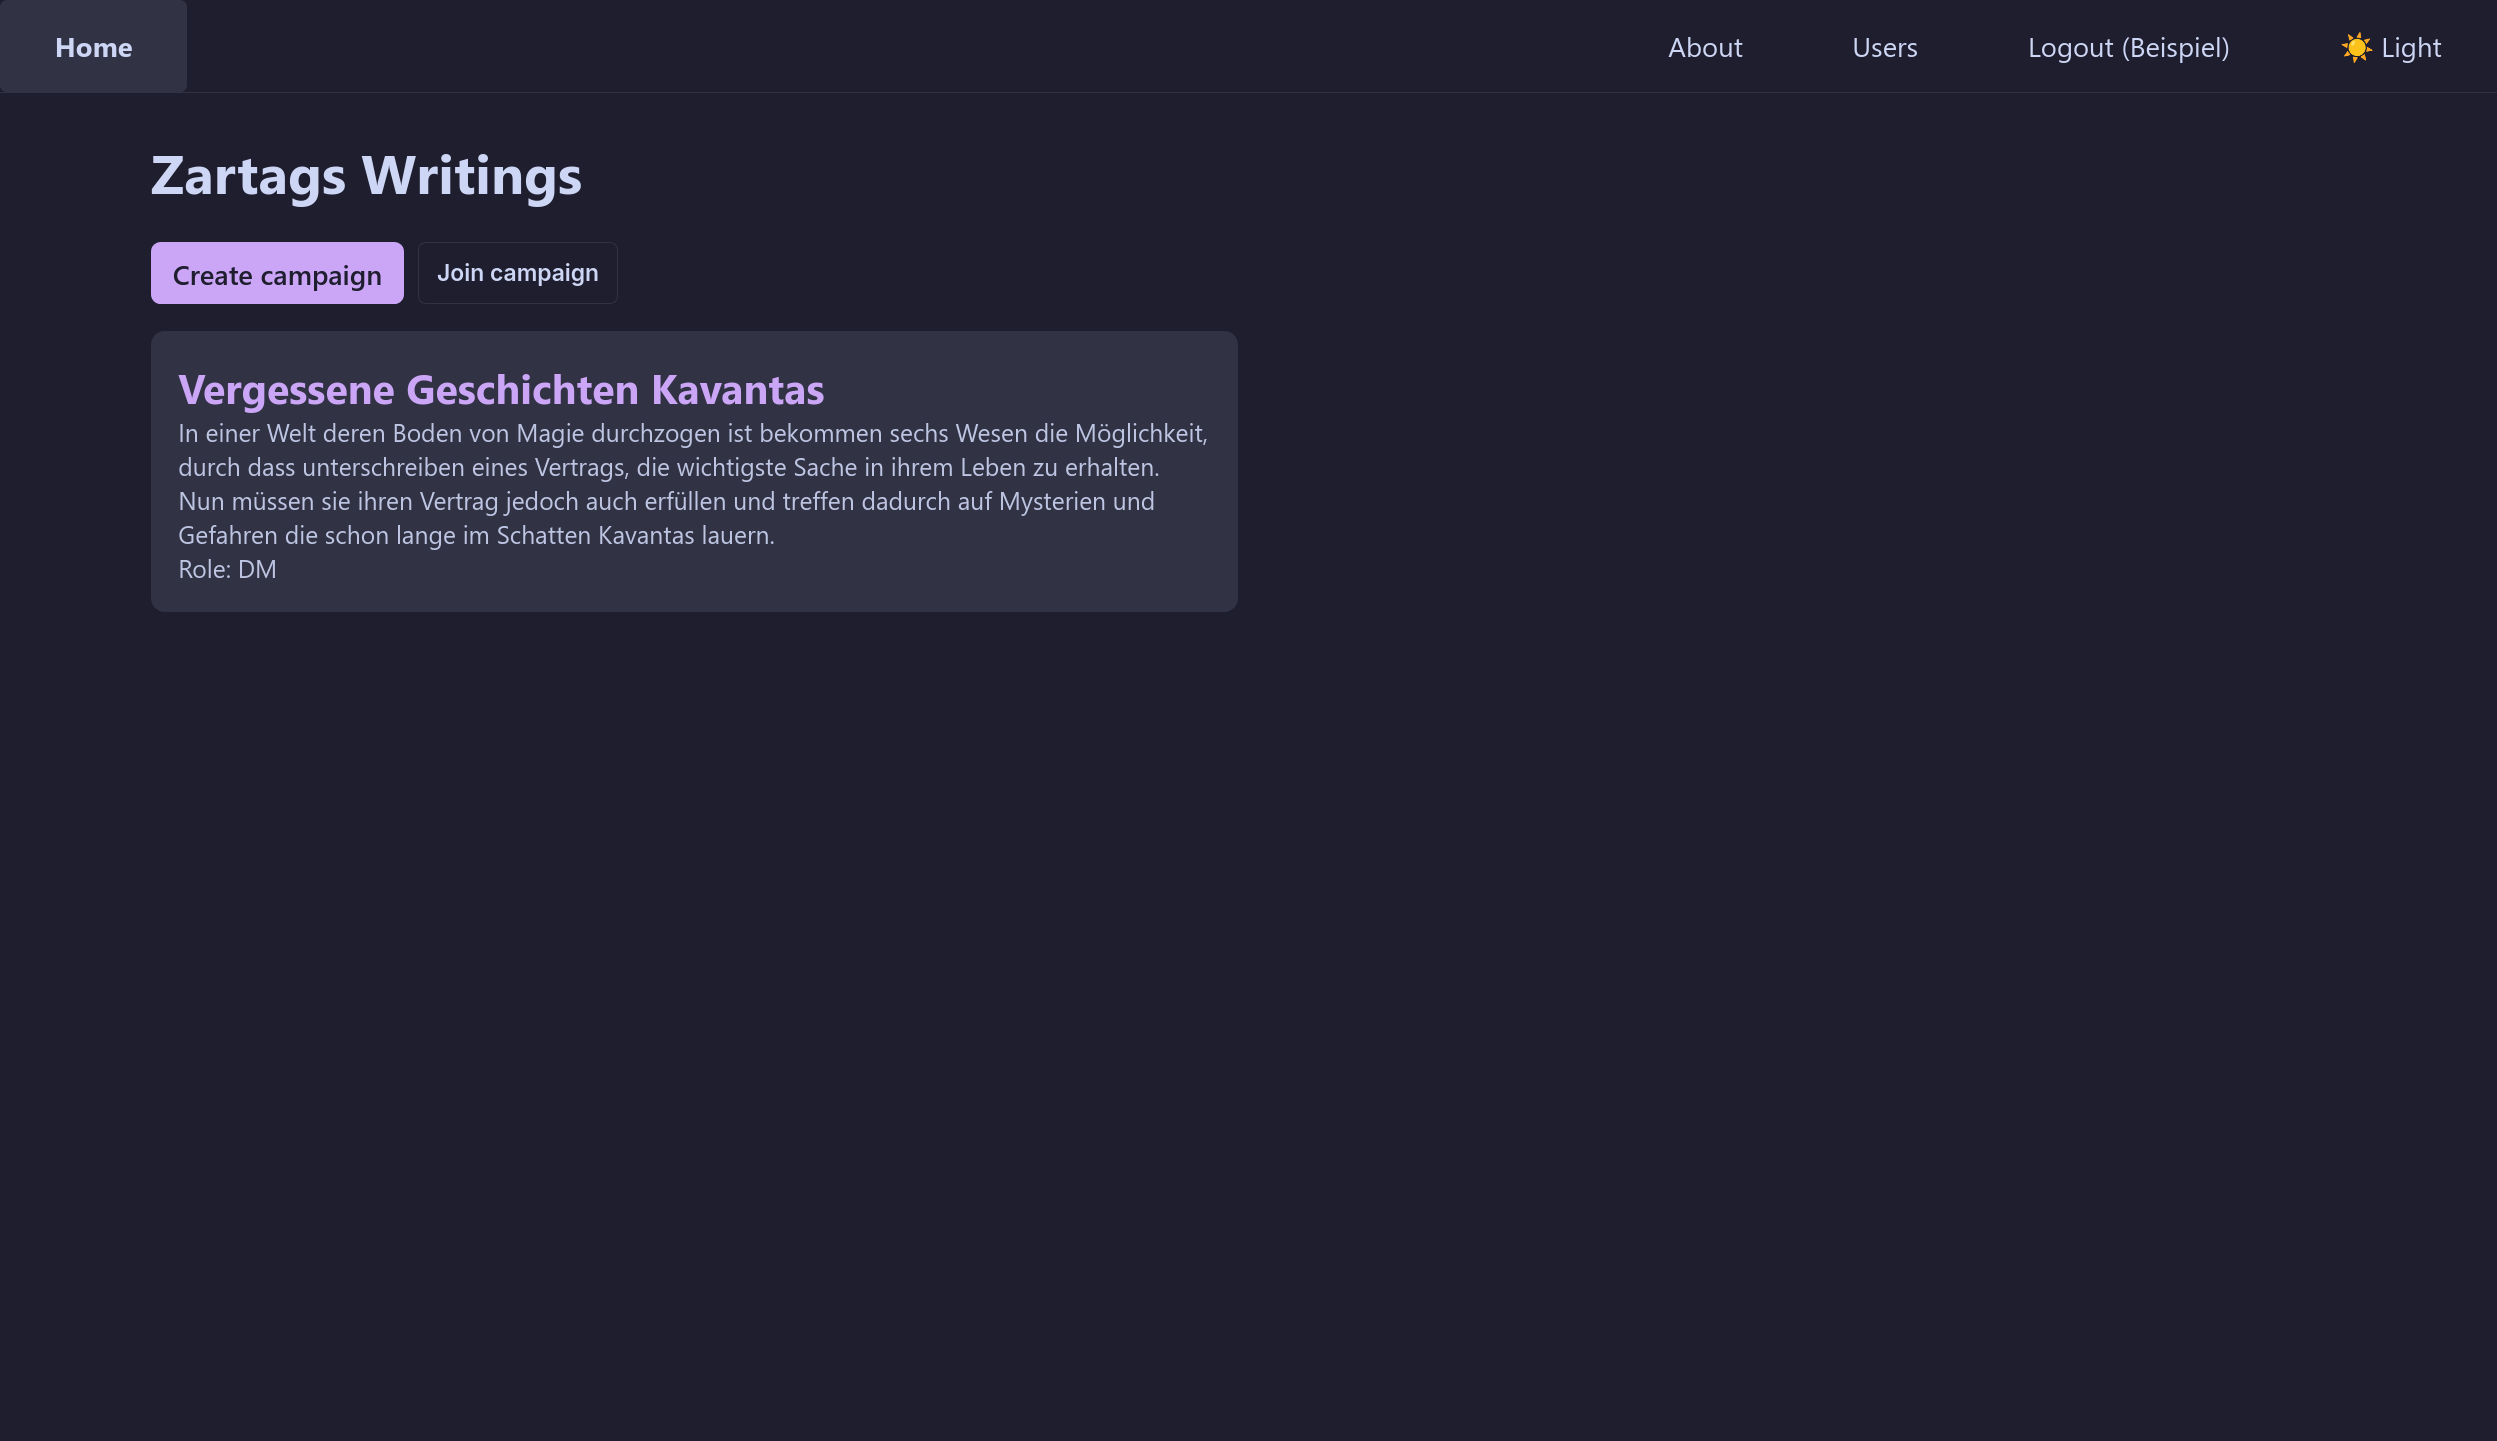
\includegraphics[width=0.92\textwidth]{media/Home_Logged_In.png}
  \caption{Startseite nach Login}
\end{figure}

\begin{figure}[H]
  \centering
  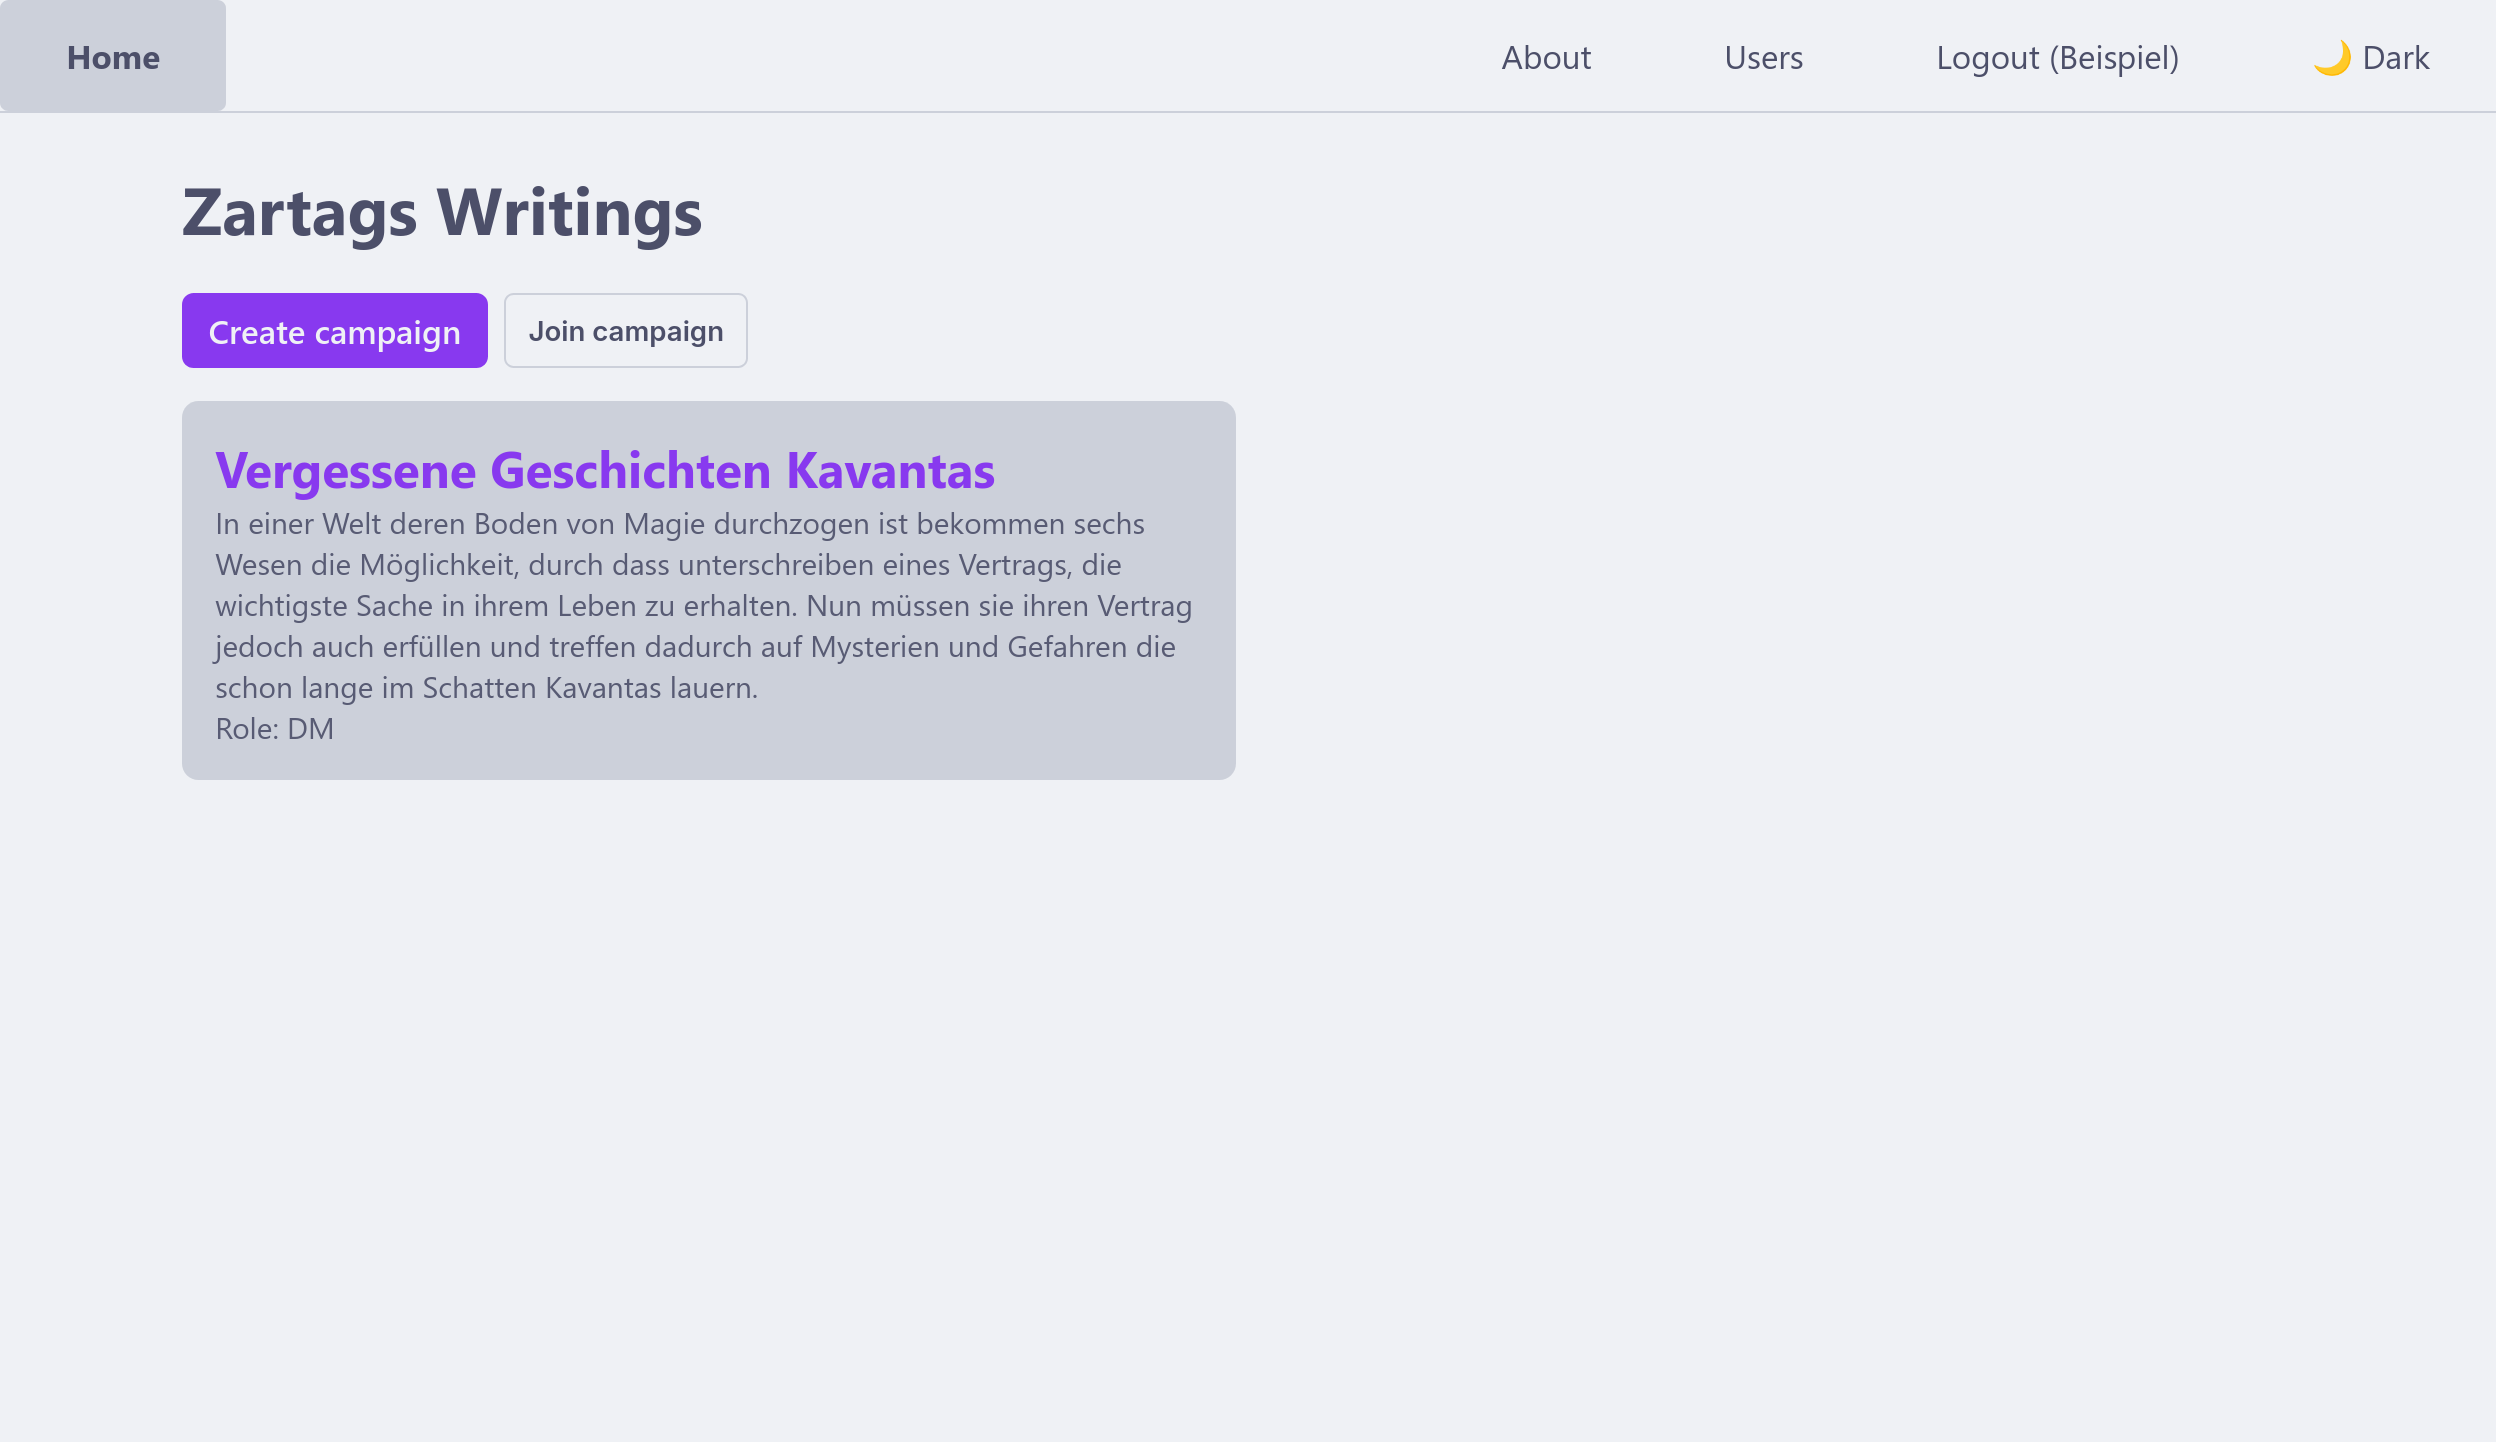
\includegraphics[width=0.92\textwidth]{media/LightMode_Home_Logged_In.png}
  \caption{Startseite nach Login im Light Mode}
\end{figure}

\begin{figure}[H]
  \centering
  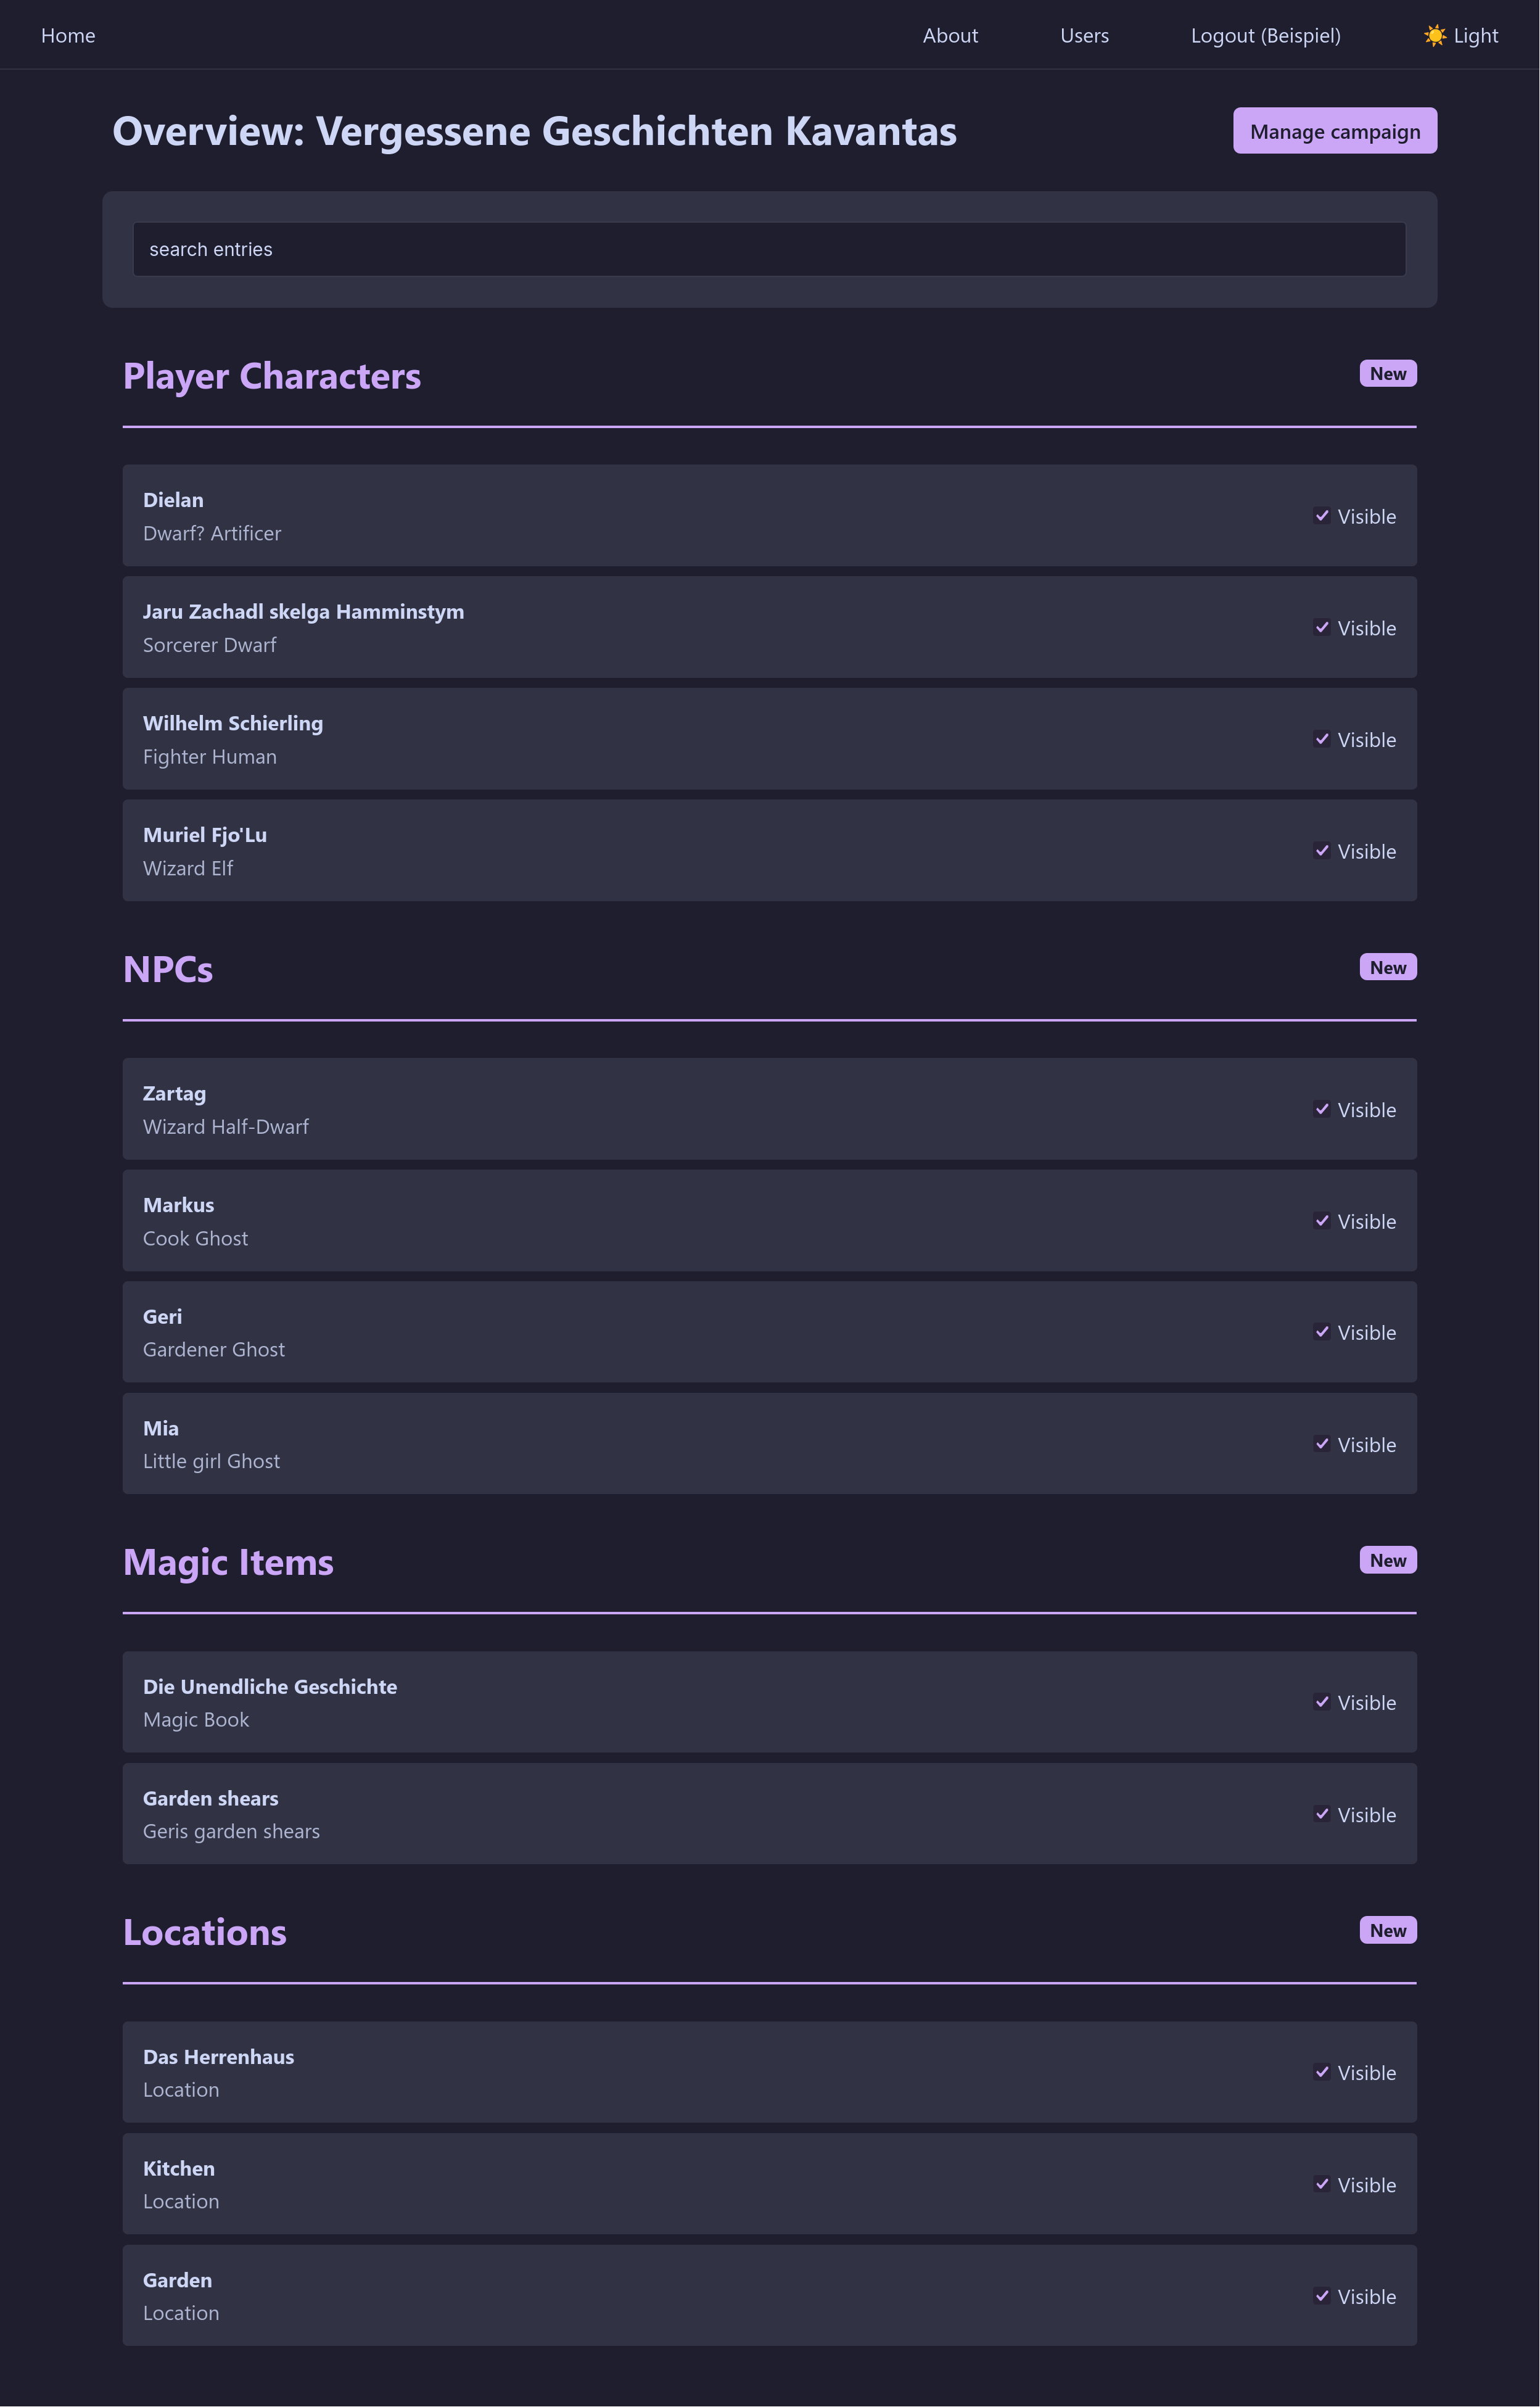
\includegraphics[width=0.92\textwidth]{media/Overview.png}
  \caption{Campaign-Übersicht mit Kategorien}
\end{figure}

\begin{figure}[H]
  \centering
  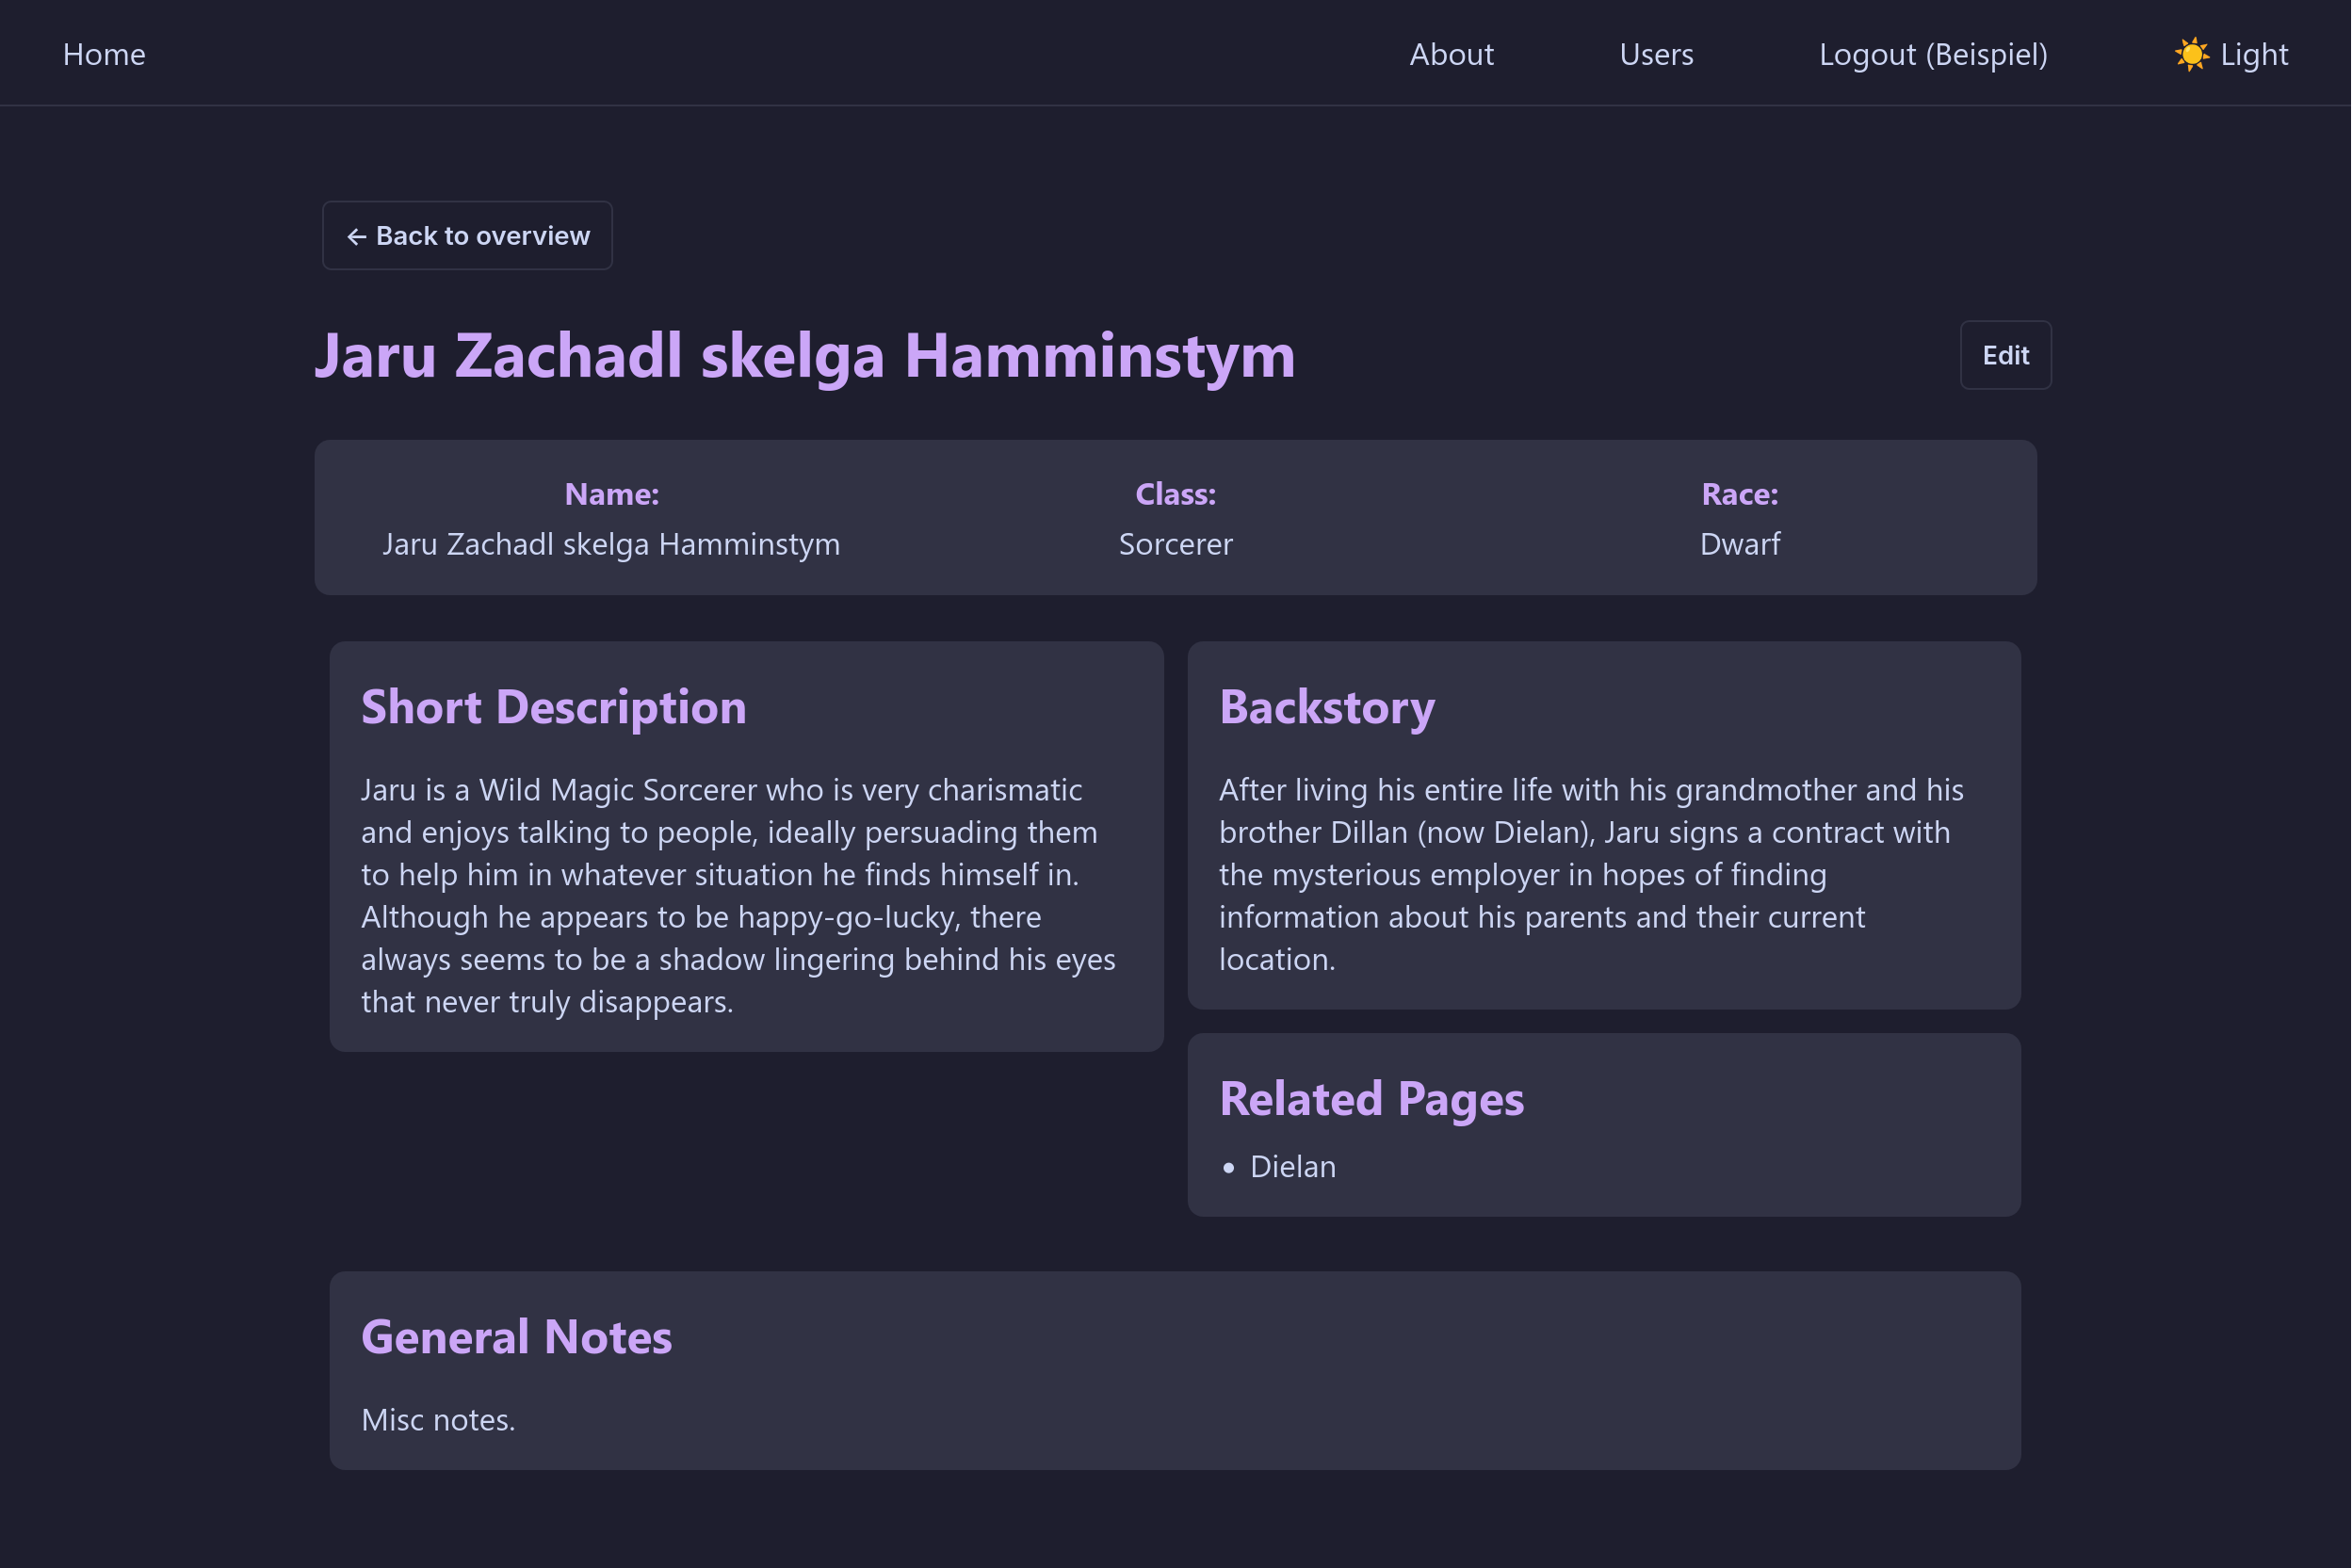
\includegraphics[width=0.92\textwidth]{media/PC.png}
  \caption{Entity-Detailansicht: Player Character}
\end{figure}

\begin{figure}[H]
  \centering
  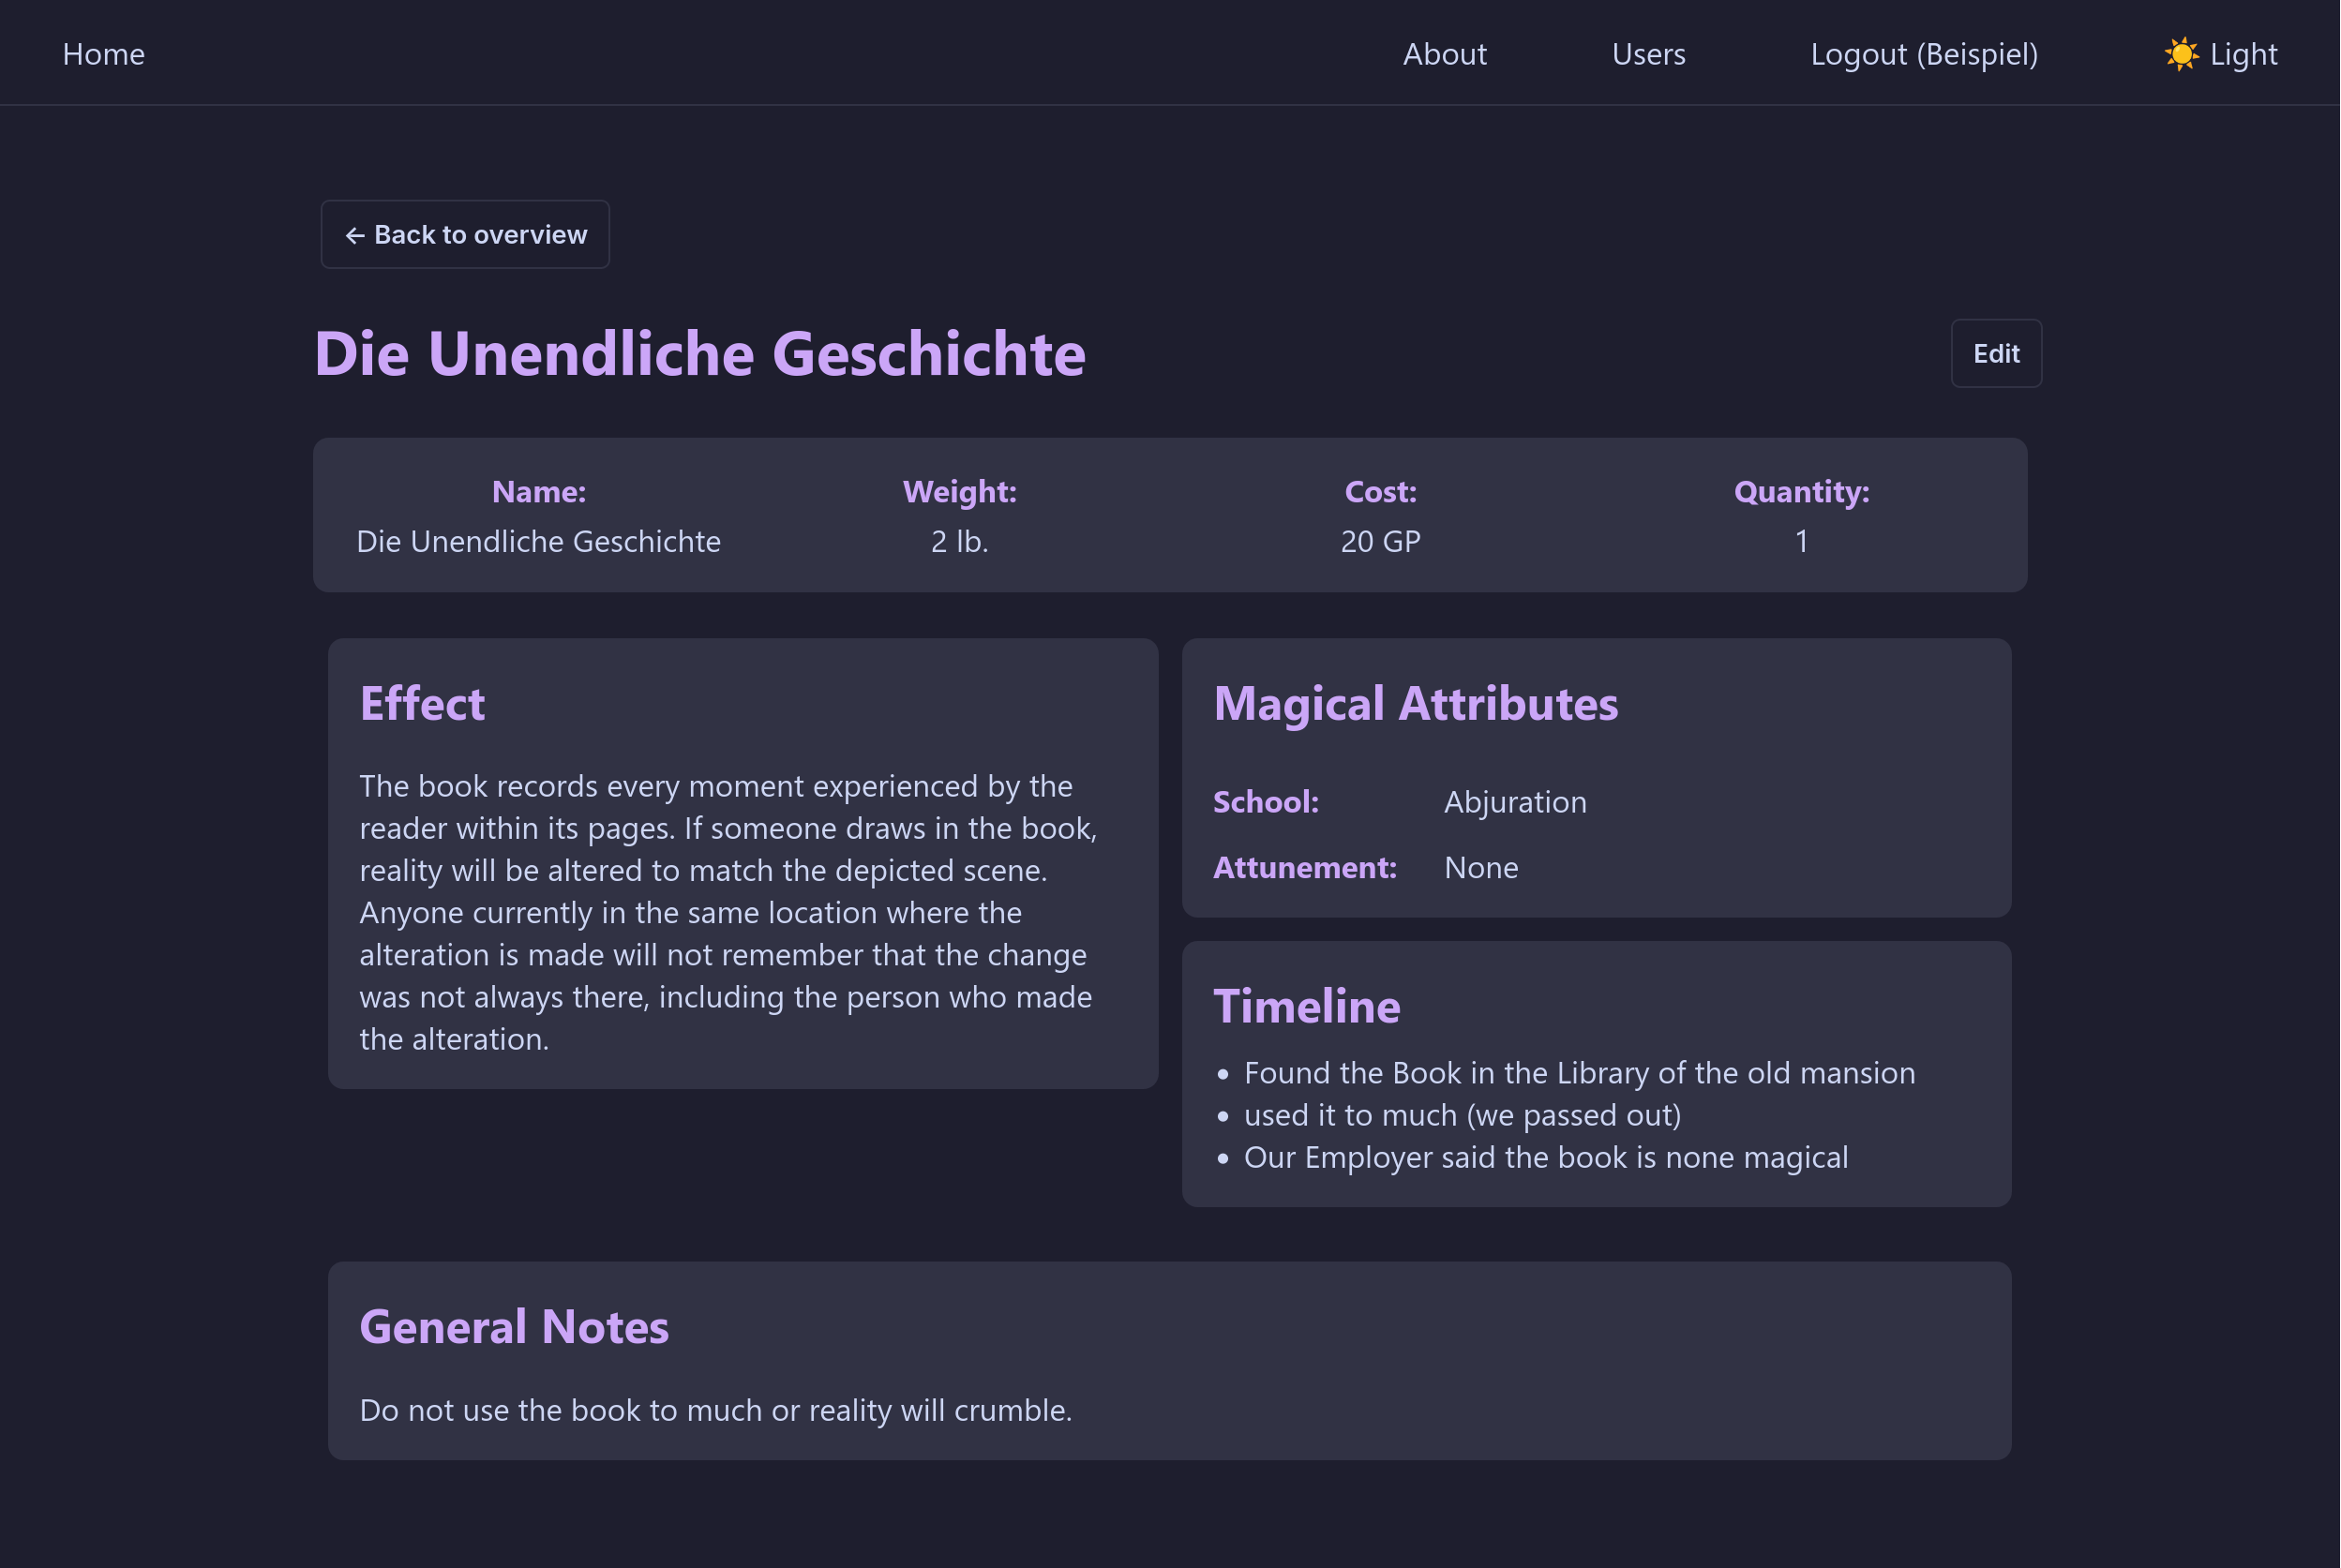
\includegraphics[width=0.92\textwidth]{media/Magic_Item.png}
  \caption{Entity-Detailansicht: Magic Item}
\end{figure}

\begin{figure}[H]
  \centering
  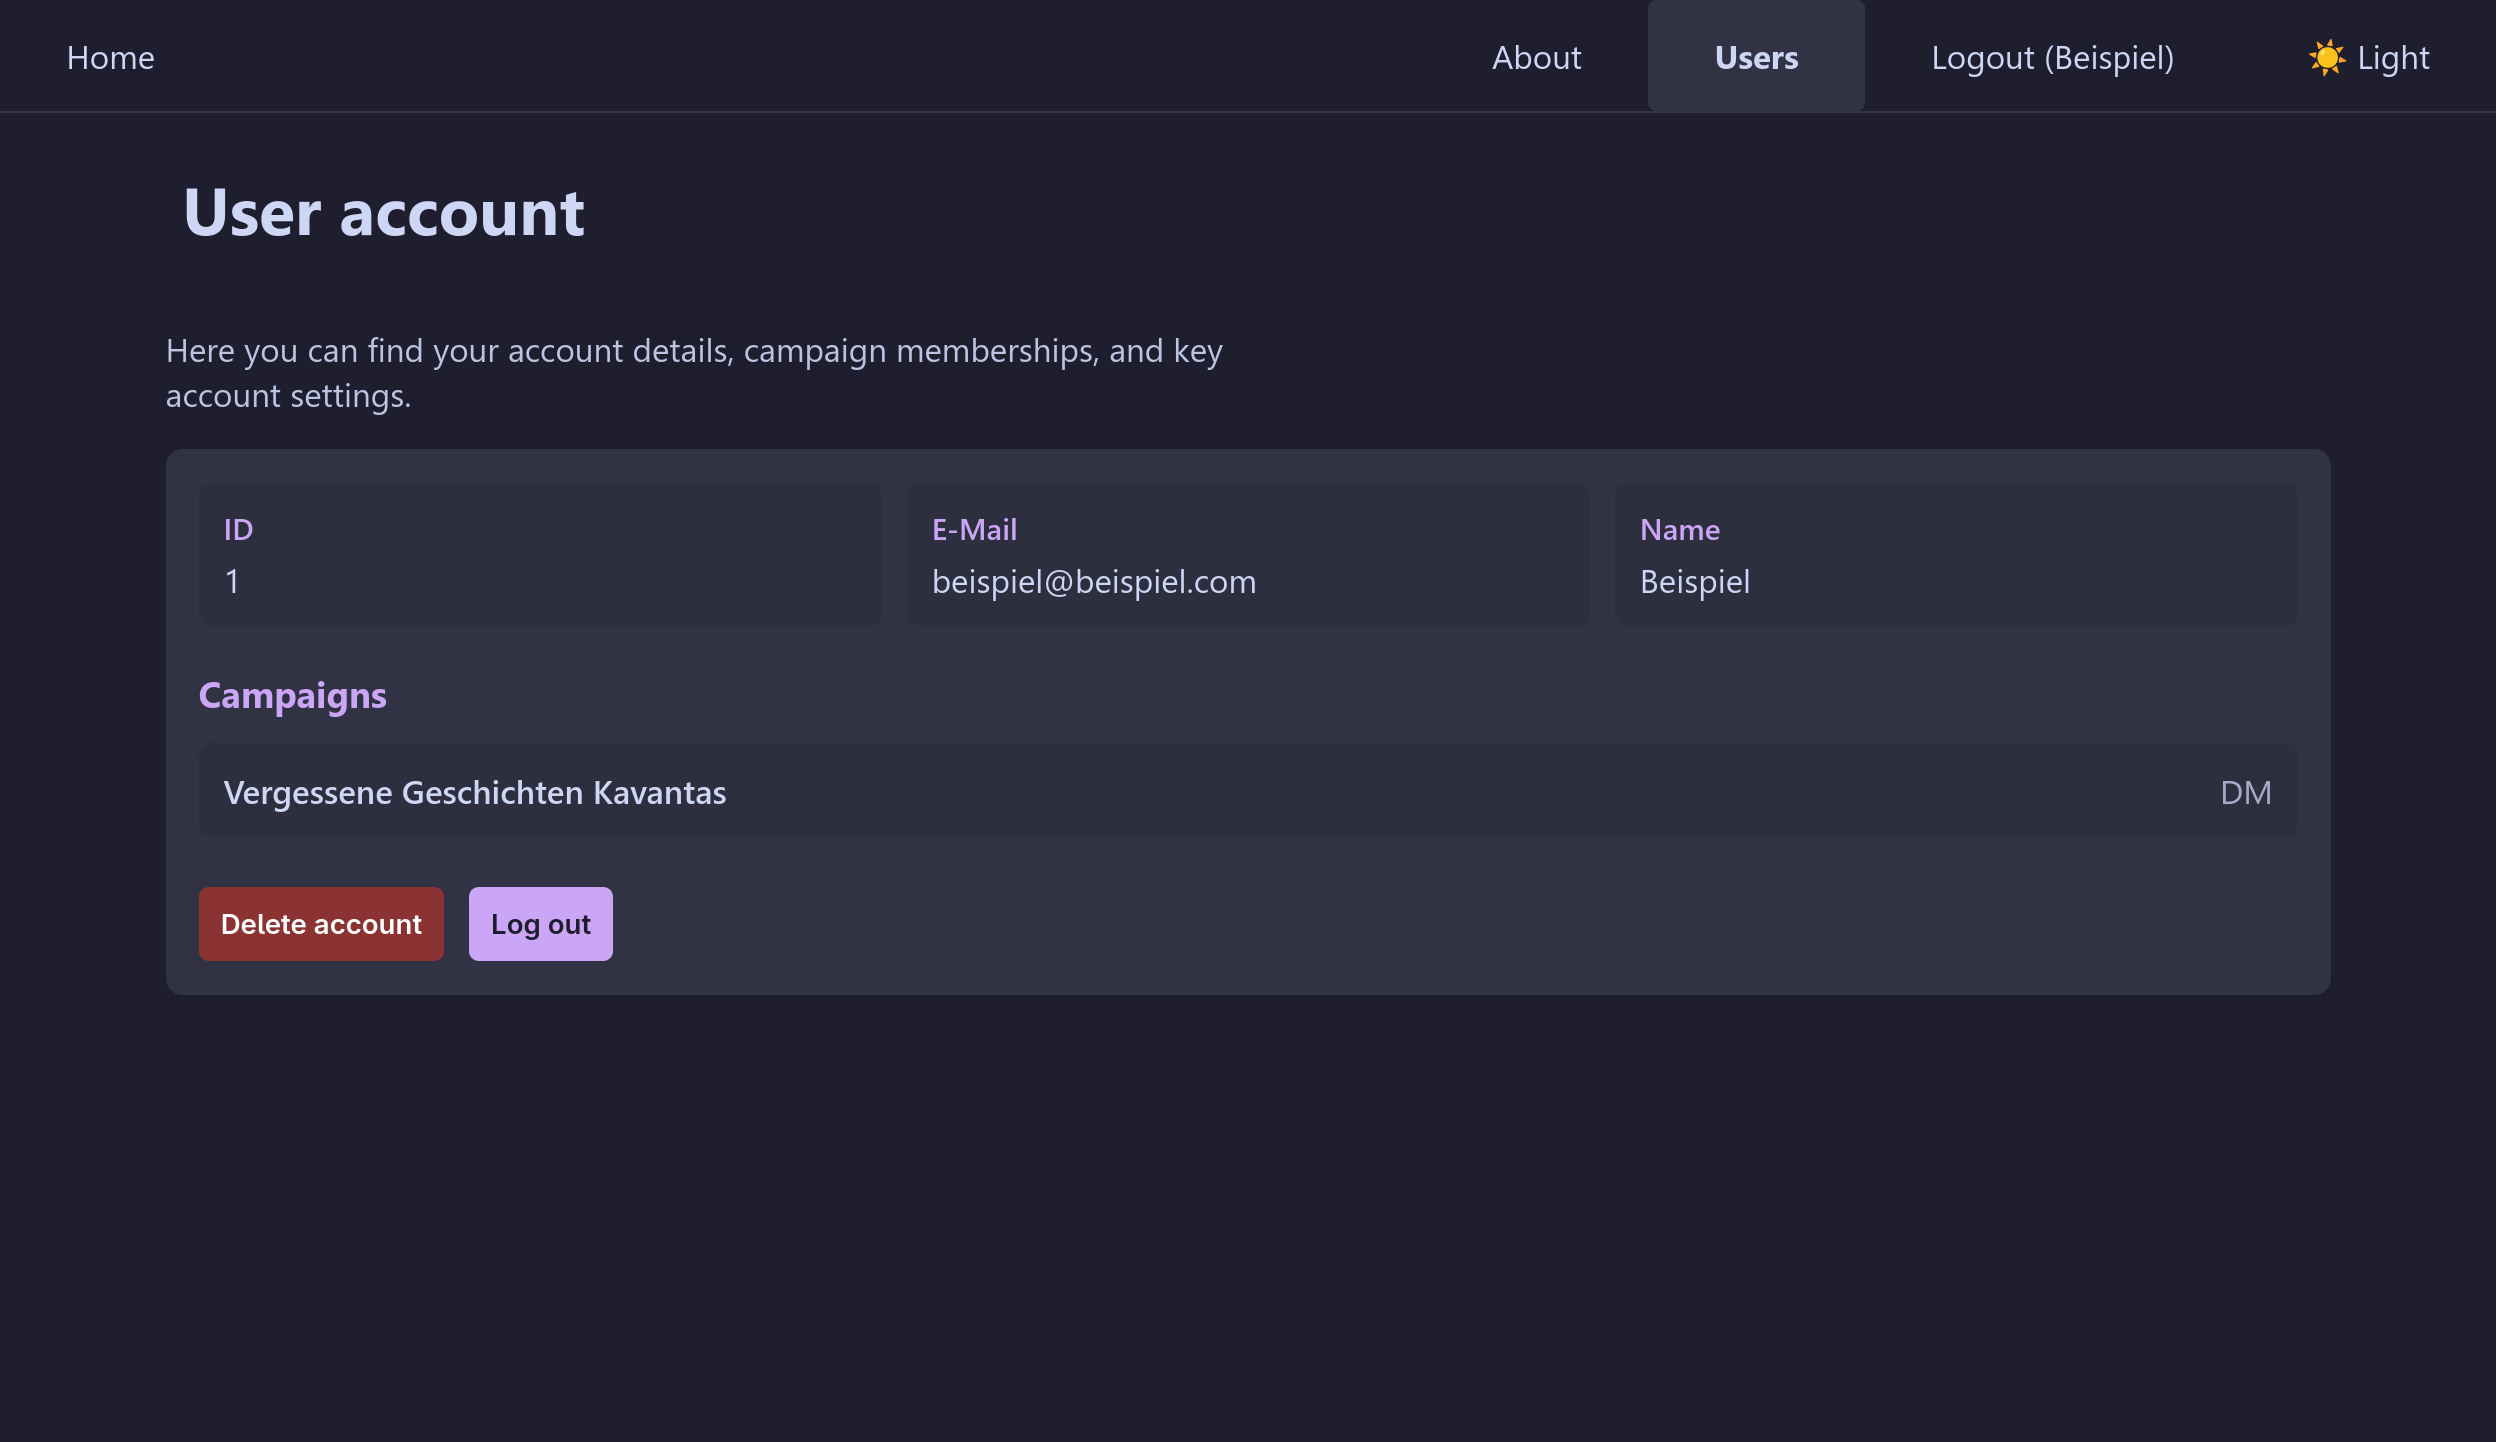
\includegraphics[width=0.92\textwidth]{media/Users.png}
  \caption{User-/Mitgliederansicht}
\end{figure}
